\chapter{Il B2B}
\begin{flushright}
	\parbox{13cm}{\small In questo capitolo viene descritto e analizzato il portale B2B, sia a livello generale che nello specifico del contesto aziendale in cui si è svolto lo stage. Vengono analizzate le funzionalità, i fattori di successo e le tecnologie utilizzate, presentandone vantaggi e svantaggi.}
\end{flushright}
\section{Il B2B in generale}
Con B2B si intende un modello per la vendita di prodotti e servizi ad altre aziende. Un portale B2B può essere considerato come un'impresa di supporto che offre ciò di cui le altre aziende necessitano per vincere la concorrenza. Il B2B, infatti, offre prodotti grezzi, servizi o articoli in stock con prezzi molto vantaggiosi rispetto alla usuale vendita al pubblico, in quanto venduti il più delle volte direttamente dalla compagnia che li produce. Al contrario, nei portali B2C destinati al cliente singolo, il prodotto finito viene venduto con un prezzo che rispecchia tutte le piccole transazioni avvenute per la composizione dello stesso: l'azienda A che produce automobili ha dovuto acquistare i bulloni dall'azienda B, le vernici dall'azienda C e il vetro dei finestrini dall'azienda D. Tutti questi acquisti da terzi aumentano di fatto il costo dell'auto finale, che dovrà di per sè garantire la copertura delle spese ed un guadagno per il venditore.

Come qualsiasi altra attività commerciale, il modello B2B richiede una attenta pianificazione. Esso tipicamente fa affidamento su un rapporto solido che il team di vendita instaura con il cliente, mentre quanto inerente la promozione commerciale può includere pubblicità in riviste commerciali, \textit{convention} e conferenze, \textit{marketing} digitale (pubblicità online, tecniche SEO, newsletter) ed altre tecniche di sensibilizzazione tradizionali.

\subsection{Il B2B come e-commerce}
Con la diffusione del web e la rivoluzione digitale, è emerso un nuovo settore definito B2B \textit{e-commerce}. Tramite portali online, le compagnie hanno iniziato a vendere direttamente ad altre aziende, così come a condividere i dati e informazioni riguardo ai prodotti ed ai servizi in modo facile e rapido. Un portale web è infatti sempre raggiungibile e permettete una diffusione immediata
delle informazioni.

Parlando di B2B \textit{e-commerce}, possono essere individuate tre categorie principali:
\begin{description}
	\item[Siti web] Molte aziende necessitano di raggiungere specificatamente altre aziende e i loro impiegati. Il sito web può rappresentare il punto d'entrata di una rete esclusiva riservata ai clienti o agli utenti registrati, o di una rete interna per l'azienda stessa. Le attività possono inoltre vendere direttamente dal sito prodotti che di fatto non richiedono di essere visti dal vivo o provati prima dell'acquisto.
	
	Un esempio sono i B2B che vendono a loro volta B2B, componibili direttamente dal cliente, tramite strumenti di composizione, template, accesso al database, metodologie per le \textit{best practice} e integrazioni per il pagamento.
	
	\item[Fornitura e offerta] Conosciti come \textit{e-procurement}, questi siti sono di solito destinati ad un mercato di nicchia. Un agente può acquistare materiale dal fornitore, richiedere una proposta di vendita ed anche effettuare offerte per comprare ad un prezzo specifico.
	
	I portali delle industrie specializzate o a sviluppo verticale forniscono una sottorete informativa per la specifica industria, come ad esempio le industrie per la sanità, di costruzioni o di altri mercati specifici.
	I portali verticali hanno uno scopo più ampio rispetto ai siti web tradizionali, ma supportano comunque la vendita.
	
	I siti di intermediazione soddisfano i bisogni delle aziende per la fornitura e la richiesta in altro modo: questi siti agiscono come intermediari tra chi fornisce il servizio e il cliente potenziale.
	
	\item[Infomediari] La categoria finale è per i siti informativi, o \virgolette{infomediari}, che forniscono informazioni specializzate per specifiche aziende. Questi portali sono spesso usati come siti organizzativi per gli standard commerciali e industriali.
\end{description}

\subsubsection{Funzionalità base}
Per essere un buon portale, un B2B deve includere alcune funzionalità fondamentali che ne determinano il successo. Queste comprendono ad esempio la gestione dell'ordine, la visualizzazione dei prodotti e la gestione dei clienti. Vi sono poi aspetti legati all'usabilità, come la semplicità nella creazione dell'ordine e l'efficienza nella ricerca di elementi come prodotti o clienti, ed altri inerenti le tecniche SEO.

\paragraph{L'ordine}
L'ordine è l'elemento alla base del B2B. Lo scopo primario di gran parte dei portali B2B è semplificare i processi interaziendali di fornitura e acquisto. L'ordine è anche l'entità più complessa che il B2B gestisce: vi sono infatti moltissimi fattori che dipendono non solo dall'azienda che ne dispone, ma anche dalle leggi statali e continentali in vigore, che possono cambiare anche frequentemente. Si pensi ad esempio all'\Gls{IVA}, una tassa applicata solo in alcuni Paesi, con regole e percentuali differenti. Un buon B2B deve essere in grado, soprattutto se destinato ad un mercato internazionale, o comunque in espansione, di gestire tutte queste variabili, a seconda di dove sta chi vende e chi compra. Non a caso una azienda per la gestione commerciale-amministrativa degli ordini necessita e si avvale di software gestionali, creati appositamente per questo scopo. Il B2B deve quindi essere in grado di riportare le logiche del gestionale nel web, rispettando le convenzioni di quest'ultimo e proponendo delle operazioni \virgolette{guidate}, in modo tale che il sistema sia utilizzabile anche da chi di gestionale ne sa poco o nulla.

\paragraph{Il catalogo}
I prodotti devono essere reperibili ed inseribili in un'ordine. Il loro dettagli deve essere chiaro: un prodotto è sempre caratterizzato da un codice che lo identifica in modo univoco, e che viene spesso utilizzato per acquisti \virgolette{rapidi}, soprattutto quando vengono effettuati ordini ripetuti (un'azienda che utilizza per tutti i macchinari un certo bullone inserirà nell'ordine direttamente il codice, piuttosto che ricercare il prodotto tramite il nome \virgolette{Bullone con testa esagonale m8}).

\paragraph{Caratteristiche generali degli e-commerce}
Essendo un portale destinato agli acquisti, il B2B deve avere le funzionalità base di questa categoria: un carrello per poter raggruppare i prodotti che si vogliono comprare e sapere in anticipo il prezzo totale; un pannello di controllo per il cliente (la \textit{dashboard}) per controllare gli ultimi movimenti e il loro stato; l'accesso al profilo per la modifica di informazioni personali; la possibilità di effettuare il login, fondamentale per poter tenere traccia delle attività svolte dagli utenti. Quest'ultimo fattore svolge un ruolo importante per determinare la strategia di marketing da parte dell'amministrazione.

\paragraph{Filtri e ricerca}
La ricerca di elementi all'interno del portale è una funzionalità che non può mancare, soprattutto con un numero di elementi molto elevato, come spesso avviene nei B2B. Allo stesso modo applicare dei filtri riduce i tempi che l'utente impiega per ottenere ciò che vuole, aumentando di fatto la sua soddisfazione.

\paragraph{Altre funzionalità}
Altre funzionalità che si possono definire \textit{must-have} sono:
\begin{itemize}
	\item configurazione dell'ordine;
	\item informazioni sulla disponibilità e sulla consegna;
	\item prezzo del prodotto pensato sul cliente;
	\item sconti e promozioni;
	\item pagamenti sicuri ed in varie modalità;
	\item \textit{Search Engine Optimization};
\end{itemize}
È necessario inoltre che siano supportati tutti i browser per le versioni più recenti e che le performance del sistema siano buone, sia in termini di caricamento delle pagine, sia per quanto riguarda i tempi di esecuzione di \textit{query} di ricerca nel database.

\subsubsection{I fattori di successo del B2B}
Il commercio \textit{business-to-business} è sempre stato uno dei vantaggi principali per la predominanza delle aziende nella competizione internazionale. L'avvento di Internet e le nuove modalità di commercio e comunicazione hanno però modificato profondamente le dinamiche e i processi tradizionali per tale mercato. Da alcune ricerche sono quindi emersi i fattori critici che una azienda deve considerare per avere successo nel B2B del web: 21 elementi, suddivisi in 5 categorie (strategia di marketing, sito web, dimensione globale, fattori interni e fattori esterni). Per individuarli sono state usate alcune tecniche specifiche, come
\begin{itemize}
	\item scansione ambientale;
	\item analisi della struttura industriale;
	\item opinione di esperti del settore;
	\item analisi della concorrenza;
	\item \textit{best practice};
	\item valutazione interna;
	\item fattori di intuizione;
	\item analisi del profitto di strategie commerciali.
\end{itemize}
Per quanto invece riguarda i fattori proposti, la forza vendita gioca un ruolo centrale nello sviluppo delle strategie di mercato se viene fornita una formazione appropriata. Il coinvolgimento di fornitori e clienti, la cultura del web e l'utilizzo di entrambi i mezzi (tradizionale ed online) sono altri fattori importanti, così come la sicurezza, la fiducia e la confidenza tra il venditore ed il potenziale cliente. L'\textit{e-commerce} è come una relazione tra le parti, dove le alleanze, l'organizzazione e le comunicazioni sono rese possibili dalle nuove tecnologie.

\paragraph{Strategia di marketing}
\subparagraph{Supporto e impegno manageriale}
È richiesta la conoscenza delle potenzialità di Internet da parte del manager, che ha anche il compito di diffonderle in modo proattivo all'interno dell'azienda. L'impegno per il commercio via web aiuta a promuovere il suo sviluppo anche in altre aziende, ma richiede comunque supporto finanziario: c'è un'importante correlazione tra l'investimento effettuato ed il guadagno ottenuto. Per questo il coinvolgimento del livello amministrativo gioca il ruolo più critico.

\subparagraph{Obiettivi strategici}
Il successo dello sviluppo del web B2B dipendono da quanto chiaramente sono definiti gli obiettivi strategici per una organizzazione.

\subparagraph{Integrazione tra Internet e la strategia di marketing}
I responsabili marketing web di successo sono quelli che costruiscono un sistema in grado di integrarsi con le applicazioni esistenti e che possano offrire la formazione necessaria per il suo utilizzo. Sebbene Internet offre molti dei servizi, esso non rimpiazzerà i mezzi tradizionali: i clienti che comprano online continuano comunque a comprare attraverso altri mezzi. Pertanto, le aziende devono considerare il web-marketing come un complemento, piuttosto che un rimpiazzo. Molti clienti infatti preferiscono valutare un prodotto online e poi procedere con l'acquisto in altri modi, di persona o al telefono ad esempio.

\subparagraph{Definizione del target}
Definire chi tra clienti esterni, fornitori, venditori, rivenditori ed altri \textit{business partner} costituisce il target è una operazione primaria, in quanto determina come i canali, gli strumenti e il target stesso sono utilizzati e coinvolti.

\paragraph{Sito web}
\subparagraph{Design}
Un sito web ben progettato e con un bel design è il biglietto da visita dell'azienda nel web. La creazione di un portale richiede però un continuo sforzo per il suo aggiornamento e mantenimento, per continuare a soddisfare le aspettative degli utenti in base alle tendenze. Un ulteriore fattore è il contenuto, che deve essere di valore, accurato ed aggiornato, sia per attrarre nuovi clienti da ogni dove, sia per incoraggiarli a ritornare; le informazioni devono essere chiare e consistenti, in quanto i clienti fanno sempre una valutazione sulla loro utilità nel condurlo a prendere decisioni. La maggior parte degli utenti arriva sul web in cerca di informazioni, pertanto un portale che offre più dettagli sull'azienda e sui prodotti avrà sicuramente più successo. D'altro canto, le performance per l'accesso a tali informazioni sono un dato altrettanto importante: la progettazione del catalogo dei prodotti va sviluppata ancor prima dello stesso portale, in quanto determina la velocità di esecuzione delle \textit{query} di ricerca per migliaia di prodotti.

Vanno quindi considerate tutte le regole base di usabilità, tra cui la semplificazione della navigazione con \gls{breadcrumb} e \gls{tag}, l'interazione e la reattività verso i \gls{feedback} degli utenti, lo scambio di informazioni tra utenti e l'integrazione del web con altri canali di marketing.\virgolette{IL sito web non deve servire solamente come interfaccia di raccolta ordini ma ha anche un alto valore aggiunto per il contenuto informativo}\autocite{b2bSuccessFactors}

\subparagraph{Promozione (offline ed online)}
La promozione è importante per due motivi: il proprio sito web deve essere riconoscibile rispetto a quello della competizione. Questo richiede una alta accessibilità, cosicché sia il sito che la sua pubblicità possano raggiungere il maggior numero di utenti possibile. Secondo, la promozione di un sito web  richiede le conoscenze tecniche di un esperto che sappia come l'utente medio trova usualmente i contenuti su Internet.

\paragraph{Fattori globali}
\subparagraph{Comprensione dell'ambiente esterno}
Un sito dovrebbe rispettare il sistema degli stati in cui è utilizzato. Vanno quindi studiati gli ambienti, incluse le regolazioni del commercio e le modalità di spedizione, per comprendere i vantaggi dei prodotti e dei servizi locali. Il mercato internazionale richiede che vengano effettuate molte considerazioni gestionali e di pianificazione, tra cui lo standard dei prodotti locali, i prezzi di mercato, i fattori competitivi, la valuta, i problemi delle modalità di pagamento, l'assistenza e i servizi offerti ai clienti e considerazioni riguardati le leggi.

\subparagraph{Risorse}
Per essere pronti all'incremento delle vendite che il portale web può portare, sono necessarie risorse, che non tutte le aziende potrebbero avere. Alcuni esempi sono la possibilità di ricevere ordini 24 ore su 24, un servizio clienti efficiente e l'esperienza per la gestione delle spedizioni internazionali

\subparagraph{Multilingua}
Uno dei problemi principali per la comunicazione a livello globale è la lingua. Per le compagnie che vogliono utilizzare il web a livello internazionale, la lingua è la sfida da superare. Per il commercio internazionale è necessario fornire una traduzione per almeno le lingue base, in modo tale da ridurre le difficoltà di comprensione per i lettori non madre-lingua.

\subparagraph{Considerazioni culturali}
Così come la lingua, anche gli altri fattori culturali devono essere riportati nel portale web. Inoltre, fornire informazioni che possano risultare interessanti da una varietà di persone con bisogni e gusti diversi può incoraggiare l'incontro tra le differenti nazioni e culture. Va considerato che anche gli elementi non testuali possono causare incomprensioni culturali, come per esempio l'uso dei colori o dei simboli delle icone (il colore bianco, che in gran parte del mondo è neutrale o addirittura elegante, in alcuni Paesi dell'Asia significa morte).

\subparagraph{Consegna internazionale}
Progettare un sistema logistico in grado di effettuare consegne in più nazioni in modo efficiente è necessario se si vuole vendere in più stati e favorisce la scalabilità per le medie aziende in espansione. Come minimo, quindi, il portale B2B dovrebbe indicare i costi e le tempistiche di spedizione verso tutti i Paesi in cui è disponibile la consegna.

\paragraph{Fattori interni}
\subparagraph{Infrastruttura tecnologica}
Affinché tutto il sistema di cui si è parlato fino ad ora funzioni correttamente, è necessario che l'infrastruttura tecnologica alla base offra buone prestazioni. Questo non è comunque l'unico aspetto da considerare, in quanto Internet per essere uno strumento utile ha bisogno che i suoi utilizzatori abbiano familiarità con il PC e sappiano apprezzare i benefici e le potenzialità che offre.

\subparagraph{Cultura interna}
Un'azienda deve comprendere e abbracciare i nuovi valori, i processi di gestione e gli stili di comunicazione che i nuovi modi di fare marketing creano. Iniziare a commerciare via web è come cominciare in un nuovo stato: la chiave del successo sta nel comprendere, apprezzare e onorare la cultura ed i protocolli di quel paese.

\subparagraph{Forza vendita}
La forza vendita ha un ruolo centrale nel successo di un portale B2B, in quanto in grado di migliorare la comunicazione, aiutando il cliente ad approcciarsi B2B e integrando nuovi strumenti di gestione dell'informazione. Le conoscenze degli addetti al marketing, inoltre, rimangono fondamentali, dato che un sito per quanto tecnologicamente avanzato non può aver successo se non rispetta le aspettative del cliente.

\subparagraph{Formazione}
Una adeguata formazione risulta importante per mantenere aggiornati gli utenti, siano essi interni od esterni, sulle nuove funzionalità e potenzialità delle tecnologie e del sistema.

\paragraph{Fattori esterni}
\subparagraph{Fiducia}
Più l'utente è cosciente di quello che sta facendo nel web, più vorrà delle garanzie. La fiducia verso un sito web sta quindi diventando la chiave che determinerà il successo o il fallimento di molte compagnie. La fiducia è ormai più importante nel monto virtuale che in quello reale, poiché le parti coinvolte in una operazione come può essere l'ordine non sono più nello stesso luogo e di certo non possono dipendere su variabili come la prossimità fisica, la stretta di mano o i segnali del corpo.

\subparagraph{Sicurezza}
Una delle preoccupazioni più diffuse nel web è la sicurezza delle transazioni finanziarie, tanto che alcuni preferiscono guardare i prodotti online, per poi utilizzare metodi offline per confermare l'ordine, come il telefono.

\subparagraph{Relazioni}
I continui cambiamenti che avvengono nel mondo dell'informatica hanno determinato un cambiamento nelle relazioni: esse si basano sempre più sull'informazione che può essere trasmessa tra aziende, piuttosto che sulle modalità con cui questa transazione avviene, come prevede invece la visione tradizionale. Svolgono un ruolo fondamentale quindi i contenuti, le tecnologie e le strategie di marketing.

\subparagraph{Infrastruttura di rete}
Uno dei fattori esterni che non dipendono direttamente dall'azienda è l'infrastruttura di rete: per sfruttare al massimo i vantaggi che il mercato virtuale offre, è necessaria una infrastruttura in grado di supportare le novità che il settore propone. 

\subparagraph{Coinvolgimento del cliente}
Come ultimo punto, ma non meno importante, è il coinvolgimento del cliente in questo tipo di attività. Le aziende dovrebbero impegnarsi a motivare i clienti ad effettuare il passaggio all'ambiente online, oltre che a predisporre un sistema interno in grado di rispondere rapidamente alle richieste dei clienti.
Il modello ottimale che soddisfa a pieno i clienti si basa infatti su una infrastruttura \textit{e-business} con quattro caratteristiche: è facile da usare, ha molte funzionalità, è affidabile ed offre prestazioni elevate.

\section{Il B2B di 4words}
Il B2B di Sanmarco Informatica è un prodotto completo ed al contempo in continua evoluzione. Svolge tutte le funzionalità base che un buon B2B dovrebbe avere e si integra pienamente con gli altri servizi dell'azienda, in particolar modo con il gestionale, agevolando così attività quali l'inserimento e la gestione degli di ordini, la gestione dei documenti e degli appuntamenti, la visualizzazione del catalogo, la configurazione di prodotti. Il B2B è fornito in varie versioni per adattarsi meglio alle esigenze dei clienti:
\begin{itemize}
	\item versione standard (il più diffuso);
	\item versione con web-services;
	\item versione moda.
\end{itemize}
In questa relazione viene trattata solamente la versione standard, l'unica su cui si è incentrato lo stage, mentre verrà solamente presentata la versione con web-services.

Ogni B2B venduto è personalizzato, anche solo in minima parte, secondo le richieste del cliente. È raro dunque incontrare due portali identici, poiché per quanto essi possano assomigliarsi per forma e contenuti, vi sono sempre delle funzionalità da una parte che l'altra ha, per scelta del cliente, nascoste.
Esistono versioni molto basilari, in cui viene personalizzato solamente l'aspetto o, ad esempio, il menu, ed altre in cui ritrovare lo standard è quasi un'impresa. Molto spesso l'utilizzo sempre più massivo del portale fa sì che sorgano proposte da parte dell'utilizzatore, che vede nel B2B la soluzione per snellire alcune pratiche altrimenti richiedenti l'uso del gestionale.

\subsection{Funzionalità principali}
In generale, il portale è composto da moduli componibili, in modo tale da essere di per sè un prodotto funzionante, ma anche facilmente personalizzabile secondo le necessità del cliente. I moduli principali sono quello dell'ordine, delle interrogazioni, l'area amministrativa, l'area dei documenti e l'agenda. Tutte queste aree sono attivabili o disattivabili per ogni utente, a seconda del suo gruppo di appartenenza. 

\subsubsection{Abilitazioni e permessi}
Una delle funzionalità principali è infatti la caratterizzazione degli utenti per ruoli. Ad ogni ruolo può essere associata un'abilitazione differente, in modo tale da adattare l'esperienza di navigazione per ognuno di essi. Si considerino per esempio gli amministratori, gli agenti di vendita e i clienti: sono tre tipi di utenza, ai quali però vanno mostrate aree differenti. Gli amministratori possono avere il controllo su tutto, in particolar modo sulle configurazioni. Sono in grado quindi di creare, modificare ed eliminare utenti, bloccarli o sbloccarli, gestire gli ordini, creare, modificare e rimuovere abilitazioni con i relativi permessi, e molto altro. L'amministratore di fatto ha il controllo completo del B2B, può arrivare a qualsiasi area, anche quelle a più basso livello, come la creazione delle connessioni ai database. L'agente di vendita potrebbe invece poter solamente creare ordini, modificandoli fin tanto che non sono inviati, creare e gestire i propri clienti, senza vedere quelli di altri agenti, così come per gli appuntamenti. La navigazione dell'agente è quindi totalmente focalizzata sulla sua funzione all'interno dell'azienda e come nel sistema tradizionale, egli non ha accesso a informazioni riguardanti suoi co-ruolo. Possono fare eccezione i capogruppo, ovvero agenti con un grado di controllo maggiore, che permette loro di controllare le attività dei subordinati. Il ruolo di cliente, infine, è generalmente quello con i permessi minori: il cliente di solito è un'altra azienda o organizzazione, che non deve quindi avere acceso ad informazioni riservate.\\
Le abilitazioni e i permessi sono di fatto del tutto personalizzabili senza l'ausilio di un tecnico 4words. Gli utenti sono inseribili, come visto, in gerarchie, che semplificano ancor di più la gestione da parte dell'amministratore, il quale in pochi passi è in grado di definire regole per molti utenti contemporaneamente. All'utilizzatore finale tutta questa serie di permessi è totalmente trasparente, in quanto non vede che esistono altre aree a lui inaccessibili.

\subsubsection{L'ordine}
Come per ogni B2B, l'ordine rappresenta il fulcro del portale e l'entità più complessa. Per rendere la creazione dell'ordine completa e al tempo stesso \textit{user-friendly}, essa è stata suddivisa in vari step che aiutano l'utente a inserire le informazioni richieste correttamente, presentandogli un numero ridotto di informazioni da fornire e, dove possibile, con aiuti, come ad esempio tramite la scelta multipla (e dunque limitata). Tramite questo \gls{wizard} è quindi possibile inviare ordini, ma anche iniziarli e lasciarli in sospeso per inviarli successivamente.

\subsubsection{Parcheggio}
Una volta inviato, l'ordine può essere inserito direttamente nel gestionale oppure ricevere dei blocchi (amministrativi o commerciali ad esempio), i quali determinano la necessità di approvazione da parte dell'ufficio relativo per il processamento dell'ordine stesso. Questo blocco è detto parcheggio e, con tutte le personalizzazioni possibili in termini di regole e modalità, è un'area molto utile in quanto velocizza alcune operazioni standard. Un tipico esempio di utilizzo è per i clienti fuori fido: a questa categoria viene permesso di fare ordini solamente a certe condizioni, verificate personalmente da alcuni addetti. Ecco quindi che il B2B permette a tali persone di accedere direttamente a tutti gli ordini sottoposti a controllo, sbloccandoli o rifiutandoli con un semplice click, con la possibilità di notificare l'utente di quanto deciso via email. Questa procedura semplifica molto operazioni che fatte direttamente nel gestionale potrebbero risultare non solo più difficoltose, ma anche meno immediate, in quanto per accedere al B2B è sufficiente un tablet o un pc connesso ad internet, mentre il gestionale è solitamente disponibile solamente dentro all'azienda.

\subsubsection{Interrogazioni}
L'area delle interrogazioni è dedicata alla ricerca di schede e informazioni riguardanti i dati inseriti dall'utente. Questi dati possono essere clienti o ordini, e sono suddivisi in varie categorie, così da permettere all'utente di trovare facilmente quello che cerca. In particolare, l'elenco dei clienti creati o utilizzati vengono raccolti in un unica videata, con tutte le loro informazioni. Anche per gli ordini esiste uno storico che indica i dettagli degli ordini inviati, bloccati o sospesi, dove è possibile applicare dei filtri di ricerca, velocizzando molto il procedimento che altrimenti sarebbe stato eseguito nel gestionale.

\subsubsection{Catalogo}
Il catalogo prodotti nella sua versione standard rispetta i requisiti del modello B2B di successo. Esso è presentato in varie modalità, secondo le convenzioni del web, tra cui la visualizzazione a lista (con più dettagli per ogni articolo) e quella a griglia, in cui hanno un ruolo importante le immagini. Questa seconda modalità è di solito rivolta a chi con il proprio B2B vuole rispecchiare gli e-commerce più famosi, come Amazon o Ebay, piuttosto che a clienti che vendono prodotti tecnici di cui sono più importanti le caratteristiche della forma. Il catalogo B2B non solo permette di effettuare ordini secondo le abitudini degli utenti (il 66\% degli utenti di Internet ha fatto acquisti online nel 2016\autocite{eurostat}), ma ha anche la funzione di sostituire i cataloghi stampati che gli agenti di vendita propongono al cliente, in quanto è legato all'utente autenticato ed è una fonte sempre aggiornata. Ad ogni prodotto è possibile associare la disponibilità, aggiornata in tempo reale rispetto al gestionale, riducendo così significativamente il numero di ordini con prodotti non disponibili o non più in produzione. Per l'agente questa è una caratteristica importante, in quanto non è più necessario mettersi in contatto con la sede centrale per conoscere cambiamenti effettuati ai prodotti, anche in termini di prezzi e listini.

\subsection{Struttura del progetto}
Passando agli aspetti implementativi, il B2B di 4words è strutturato gerarchicamente in vari progetti, con in testa alla gerarchia la versione base e al di sotto varie versioni dipendenti dalle soprastanti. In particolare la versione standard precedentemente citata è così formata:
\begin{itemize}
	\item B2B Base: costituisce gran parte del back-end dell'applicazione. Contiene pressoché tutta la logica del portale e non ha alcun tipo di riferimento al front-end. Si occupa principalmente di gestire i dati del gestionale, riproducendoli sotto forma di oggetti.
	\item B2B Prime: è il nucleo del front-end. Include le librerie grafiche e predispone la totalità delle pagine navigabili nel portale. Si occupa anche di collegare il front-end alle classi del back-end, aggiungendo o aggiustando gli oggetti per renderli usufruibili dalla parte grafica.
	\item B2B R14: costituisce l'ultima grossa release di creazione del portale e rappresenta l'ultimo strato comune a tutti i progetti. È il vero e proprio applicativo ed in esso vengono definiti i denominatori comuni per creare uno standard stabile e duraturo, oltre che compatibile con i molti moduli disponibili per l'installazione.
\end{itemize}
Questi tre progetti formano quello che si è soliti definire lo standard del B2B. Esso rende l'installazione per il cliente semplice e immediata in quanto configura già di suo la maggior parte delle funzionalità.
Da questi tre progetti si sviluppano poi una serie di moduli tra loro indipendenti, tra cui:
\begin{itemize}
	\item B2B TCE: è il modulo che integra il B2B con il configuratore di prodotto offerto dall'azienda.
	\item B2B Rest Service: include le librerie necessarie per interrogare le \Gls{API} di servizi \Gls{REST}, come ad esempio di \Gls{Magento} o \Gls{Prestashop}. È il ponte tra il B2B e i vari \Gls{CMS} disponibili online e il suo scopo è proprio quello di agevolare l'interfacciamento tra questi due tipi di contenuto.
	\item B2B Rest Client: costituisce l'interfaccia grafica dell'integrazione B2B con i servizi web.
\end{itemize}
A partire da questi progetti vengono quindi creati i prodotti finali venduti ai clienti. Ogni cliente ha il suo progetto dedicato, in quanto sorgono in continuazione nuove richieste, sviluppate quindi in un ambiente indipendente, in modo tale da non creare conflitti con implementazioni contrarie di altri clienti.

Il B2B è strutturato secondo il pattern \Gls{MVC}. Questo pattern è individuabile in più livelli:
\begin{itemize}
	\item Nell'architettura ad alto livello, il \textit{model} è composto dai componenti che contengono la logica dell'applicazione, in particolare da \textit{manager}, \textit{data provider} e \textit{program provider}; la \textit{view} è composta dal \virgolette{codice JSF}; il controller è costituito dalla FacesServlet, una \gls{servlet} che gestisce le richieste delle applicazioni web.
	\item La view del precedente livello rispecchia a sua volta il pattern, dove il \textit{model} è costituito dalle entità, la \textit{view} è composta dalle pagine \texttt{\gls{XHTML}} (le \gls{facelets}) e il controller è formato dai \textit{backing bean}.
\end{itemize}
L'architettura può quindi essere riassunta con lo schema M(MVC)C. Questa ricorsione si potrebbe protrarre anche al livello del client, aggiungendo quindi un ulteriore livello interno.

Nel B2B il \textit{model} architetturale è stato suddiviso in vari \textit{package}, citati precedentemente. I \textit{manager} contengono la logica dell'applicazione e collegano la \textit{view} ai \textit{data provider}, i quali rappresentano il \textit{data layer} nel pattern architetturale \Gls{DAO}. Questi, inoltre, possono fare riferimento al loro interno ai \textit{program provider}, i quali rappresentano l'interfaccia Java per i programmi \Gls{RPG} dell'\Gls{AS400}. Secondo le norme di programmazione prestabilite per il progetto B2B, dunque, il flusso esecutivo per una operazione che richiede la chiamata ad un programma RPG è il seguente: la pagina fa riferimento ad un metodo del \textit{backing bean}, che chiama il manager di competenza, il quale trasferisce la richiesta al \textit{data provider}, che richiama il \textit{program provider}. Il risultato della chiamata al programma torna quindi indietro attraverso \textit{data provider}, \textit{manager} e \textit{backing bean}, che effettueranno eventuali controlli e operazioni necessari. Infine, se richiesto dall'applicativo, la pagina viene aggiornata e/o nuovamente renderizzata.

Quasi la totalità delle entità concepite nel B2B 4words ha un oggetto corrispettivo nei \textit{backing bean}, nei \textit{manager}, nei \textit{data provider} e, a volte, nei \textit{program provider}. Questa suddivisione permette di applicare il \textit{single responsibility principle} (principio di singola responsabilità), secondo il quale ogni elemento deve avere una singola responsabilità, interamente incapsulata dall'elemento stesso. Ad esempio, l'entità \texttt{Order} è gestita rispettivamente nell'\texttt{OrderBck} per quanto riguarda il suo interfacciamento con le pagine JSF, nell'\texttt{OrderManager} per la logica e nel \texttt{OrderDataProvider} per l'accesso al database. Anche le personalizzazioni risultano così immediate, in quanto, per la gerarchia descritta precedentemente, è sufficiente derivare la classe che richiede la personalizzazione per usufruire di tutti i vantaggi che la struttura porta con sé, tra cui il polimorfismo.

Le pagine \texttt{XHTML} sono strutturate in modo tale da permettere il riutilizzo ove possibile, tramite template e componenti creati ad hoc per svolgere alcuni compiti specifici, come il calendario o il campo di testo per la valuta. Questo è reso possibile anche grazie all'utilizzo di JSF.

\subsubsection{Vantaggi e svantaggi}
La struttura appena descritta presenta alcuni vantaggi e svantaggi importanti.
\paragraph{Vantaggi}
Il primo vantaggio è che la suddivisione in più progetti permette che essi siano gestiti da un gruppo limitato di persone, riducendo il rischio di creare conflitti nelle modifiche contemporanee. Inoltre, ogni progetto cliente è indipendente dagli altri, e dipende solo dai pacchetti di cui necessita: non vengono installate librerie al di fuori di quelle richieste per il corretto funzionamento, mantenendo quanto si va ad installare il più leggero possibile.

La separazione in più progetti permette anche una distribuzione dei ruoli all'interno del gruppo di sviluppo: l'implementazione di nuove funzionalità generali e solitamente di grosso impatto è affidata al gruppo standard; la personalizzazione delle funzionalità esistenti e lo sviluppo di funzionalità specifiche o non comuni, che quindi risulterebbero utili a pochi, è lasciato ai sistemisti con a carico il cliente. Nel caso in cui sorgano anomalie o problematiche negli ambienti dei clienti riguardo a moduli standard, interviene l'assistenza, la quale si occupa di individuare e correggere gli errori cosicché possa essere rilasciato un aggiornamento risolutivo comune per tutti i clienti.

La struttura gerarchica fortemente basata sull'ereditarietà facilita anche chi si addentra per la prima volta in un progetto così ampio nell'individuare il flusso d'esecuzione. I passaggi e le chiamate tra metodi seguono infatti sempre la stessa linea: la pagina utilizza le proprietà dei \textit{backing bean}, i quali richiamano i \textit{manager} per le operazioni logiche, che a loro volta utilizzano i \textit{data provider} per effettuare letture e scritture del database, dai quali vengono richiamati i \textit{program provider} per le chiamate a programmi RPG. 

\paragraph{Svantaggi}
Uno degli svantaggi principali nell'utilizzo di questa struttura è che con aggiornamenti del pacchetto standard importanti, laddove il cliente ha un portale molto personalizzato, c'è il rischio che le personalizzazioni si invalidino, richiedendo di fatto un lungo lavoro di \virgolette{riporto} delle classi personalizzate per mantenerle compatibili con la nuova versione standard. Vi sono di fatto due possibilità: aggiornare l'intero pacchetto standard e modificare di conseguenza la parte personalizzata o procedere al contrario, aggiornando solamente ciò che aggiunge funzionalità o che corregge comportamenti anomali, senza modificare i metodi standard richiamati dalle classi personalizzate. Nel primo caso, come detto, il lavoro può risultare molto lungo, mentre nel secondo caso si rischia di arrivare ad uno stato di inconsistenza, dove più classi richiedono che uno stesso metodo svolga operazioni diverse, dovendo quindi comunque effettuare modifiche a svariate personalizzazioni. Tutto questo prevede anche una lunga fase di test, ai quali non viene mai dedicato il giusto tempo.

\subsection{Versionamento}
Lo strumento di versionamento utilizzato per tutti i progetti riguardanti il B2B è \Gls{RTC}. Esso si basa su IBM Jazz, una piattaforma estendibile che aiuta i team ad integrare i task durante il ciclo di vita del software. RTC è costruito su una architettura client-server ed è integrabile con molti altri prodotti, tra cui \gls{Git}, \Gls{Jenkins} e \Gls{Maven}. Per quanto riguarda la funzione di versionamento, RTC è così strutturato: sul server sono presenti gli \textit{stream}, dei contenitori contenenti uno o più progetti, accessibili solamente tramite invito. Agli utenti invitati vengono attribuiti uno o più ruoli, ad esempio \textit{scrum master} o membro del team (solitamente lo sviluppatore senza permessi amministrativi), che determinano i permessi a loro associati. 

RTC è strutturato secondo lo schema in \hyperref[fig:rtc-struttura]{figura \ref{fig:rtc-struttura}}.
\begin{figure}[H]
	\centering
	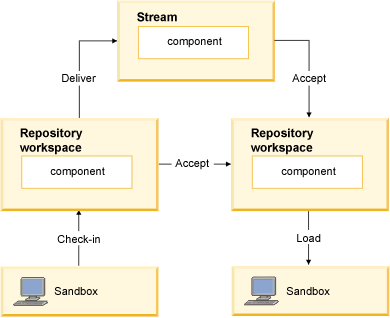
\includegraphics{Immagini/rtc-struttura.png}
	\caption{Struttura del sistema di versionamento RTC}
	\label{fig:rtc-struttura}
\end{figure}
Il sistema è centralizzato sullo \textit{stream}, sul quale confluiscono tutte le modifiche e dal quale gli utenti scaricano i progetti. Vi è poi un livello intermedio, appartenente ai singoli utenti, che si trova sul server e permette agli utenti di salvare le proprie modifiche online, così da non correre il rischio di perderle a causa di malfunzionamenti hardware. Questo strato è chiamato \textit{repository workspace}. Infine, il livello più basso è quello che risiede in locale, nel PC in cui si lavora. Le operazioni tra livelli hanno nomi specifici: il \textit{check-in} è il trasferimento delle modifiche dal \textit{workspace} locale a quello remoto; con \textit{deliver} si intende il trasferimento delle modifiche dal \textit{workspace} remoto allo \textit{stream}. Con questa operazione le modifiche diventano effettive e scaricabili da tutti gli utenti, i quali devono accettarle (\textit{accept}) per trasferirle al proprio \textit{workspace} remoto e quindi riportarle in ambiente locale tramite l'operazione \textit{load}.

Le funzionalità principali di RTC utilizzate per lo sviluppo del B2B sono:
\begin{itemize}
	\item \textit{work item}: sono il meccanismo sui cui si basa RTC per tracciare e coordinare i \textit{task} di sviluppo e il flusso di lavoro. Sono il collegamento tra varie funzionalità di RTC, come le \textit{build} e i \textit{change set} (l'insieme delle modifiche associate, appunto, al\textit{ work item}). I \textit{work item} possono assumere una categoria diversa a seconda del loro contesto, come ad esempio \virgolette{implementazione} o \virgolette{bug}, per distinguere se le modifiche rilasciate costituiscono una nuova implementazione o risolvono una anomalia presente nel codice.
	\item Controllo dei sorgenti: è un sistema di controllo di versione costruito sulla piattaforma Jazz. Offre supporto per lo sviluppo parallelo con modello agile, integrando anche un sistema di gestione degli errori.
	\item Pianificazione: il componente per la pianificazione fornisce uno strumento di assistenza nell'organizzazione e svolgimento di progetti agile e non. Per lo sviluppo agile permette di salvare lo stato dei lavori ad una certa \textit{release} o ad uno \textit{sprint} e di tenere traccia del progresso durante le iterazioni, bilanciando il lavoro tra gli sviluppatori. Questo modello viene utilizzato soprattutto per lo sviluppo dei progetti standard, in quanto le personalizzazioni sono solitamente affidate ad una o due persone.
\end{itemize}
RTC è usato tramite la sua integrazione per Eclipse, l'IDE di sviluppo del B2B. Un tipico esempio di utilizzo di RTC è presentato in \hyperref[fig:rtc]{figura \ref{fig:rtc}}.
\begin{figure}[H]
	\centering
	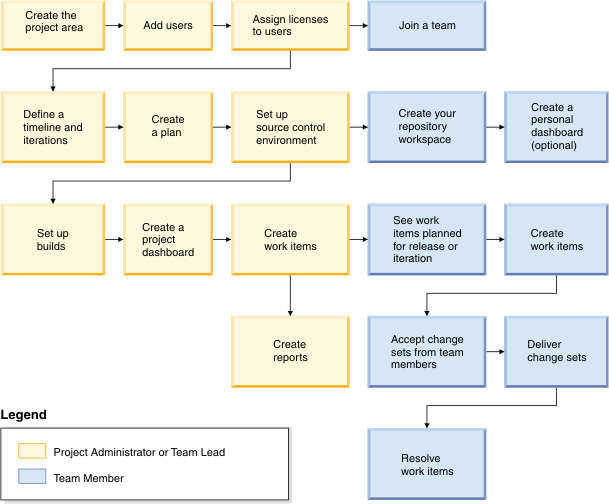
\includegraphics[width=14cm]{Immagini/rtc-task-flow.png}
	\caption{Flusso di lavoro tipico di RTC}
	\label{fig:rtc}
\end{figure}

\subsubsection{Vantaggi e svantaggi}
Per analizzare i vantaggi e gli svantaggi di questo strumento, viene fatto un confronto con Git.
\paragraph*{Modello di repository}
\begin{itemize}
	\item[\textbf{Git}:] distribuito. I vari \textit{repository} agiscono come peer e gli utenti hanno solitamente una copia locale con tutta la storia dei cambiamenti in aggiunta a quella in cui stanno lavorando.
	\item[\textbf{RTC}:] \textit{client-server}. Gli utenti accedono ad un \textit{repository} principale (lo \textit{stream}) tramite un \textit{client}; tipicamente in locale viene conservata solamente la copia di lavoro del progetto e i cambiamenti devono essere inviati allo \textit{stream} prima di essere propagati agli altri utenti.
\end{itemize}
Il vantaggio che un sistema centralizzato ha rispetto ad uno distribuito è che lo spazio richiesto per mantenere in locale la copia del progetto è limitato alle sole dimensioni dei file dello stesso. Questo comporta però la necessità di essere collegati in rete anche solo per consultare le modifiche apportate ad un file, che non sono disponibili in locale. Questo comportamento presenta anche il seguente svantaggio: se per un progetto di un cliente lo standard rilasciato non è aggiornato con le ultime modifiche presenti sullo \textit{stream}, un nuovo componente del team che dovrà lavorare su quel progetto scaricherà una versione diversa da quella del cliente. Non c'è pertanto la sicurezza che quanto modificato funzioni effettivamente, se non aggiornando il pacchetto standard interamente, operazione rischiosa se fatta da tale nuova persona, che può non conoscere approfonditamente tutte le personalizzazioni del cliente.

Per ovviare a questo problema sono possibili varie strategie: la prima è un passaggio manuale del \textit{workspace} locale del progetto tra lo sviluppatore che si è occupato del cliente in questione e il nuovo arrivato. Questo, oltre a non essere sempre possibile, presenta alcuni problemi: nel caso in cui non si voglia aggiornare tutto il pacchetto standard del cliente con la versione corrente dello \textit{stream}, ma solo con alcune modifiche (correttive ad esempio), diventa necessario comunicare agli altri detentori del progetto quali work item sono stati scaricati o che modifiche sono state fatte, in modo tale che possano essere riportate in tutte le versioni locali. Una operazione simile è del tutto contraria alle logiche e alle regole dei sistemi di versionamento. La seconda opzione è quella di creare nello \textit{stream} dei clienti una copia dei progetti standard, cosicché ogni progetto cliente sia indipendente. Questa strategia richiede però un impegno maggiore, soprattutto in termini di manutenibilità. Una ulteriore possibilità è quella di creare delle \textit{release} per i vari progetti clienti, in modo tale che il nuovo componente possa scaricare lo \textit{stream} standard alla \textit{release} del cliente. Questa andrà revisionata man mano che vengono effettuati gli aggiornamenti. Lo svantaggio di questa modalità è che nello \textit{stream} del progetto standard emergono tante \textit{release} quanti sono i clienti e, per numero molto ampio, potrebbe appesantire lo \textit{stream} stesso. Nonostante ciò, quest'ultima strategia sembra essere la più idonea per gestire questo genere di situazioni.

\paragraph*{Gestione della concorrenza}
\begin{itemize}
	\item[\textbf{Git}:] \textit{merge}. Le modifiche possono avvenire in modo concorrente e l'utente è avvisato di possibili conflitti quando vuole eseguire un aggiornamento del \textit{repository}. Questo conflitto può essere risolto direttamente dal sistema o manualmente dall'utente per poi inviare la nuova versione agli utenti.
	\item[\textbf{RTC}:] \textit{merge} o \textit{lock}. Sebbene sia disponibile anche il modello \textit{lock}, in cui le modifiche non sono permesse finché l'utente non chiede e riceve il \textit{lock} esclusivo sul file, per il B2B è utilizzato il sistema di \textit{merge}, come in Git.
\end{itemize}
La scelta di utilizzare il modello di \textit{merge} è sicuramente la migliore, in quanto permette di collaborare contemporaneamente sugli stessi file, il che rappresenta un notevole vantaggio nello sviluppo dei progetti.

\paragraph*{Metodo di salvataggio}
\begin{itemize}
	\item[\textbf{Git}:] \textit{snapshot}. Vengono salvati per ogni versione i file interi, compressi per ottimizzare e ridurre la dimensione complessiva dell'albero.
	\item[\textbf{RTC}:] \textit{change set}. Vengono salvati solamente i cambiamenti tra revisioni.
\end{itemize}
Sebbene con il modello di salvataggio utilizzato da Git le varie versioni dei file sono accessibili in modo immediato, il modello a \textit{change set} richiede di fatto meno spazio sul disco. Nello specifico, nello sviluppo del B2B risulta più un vantaggio questo risparmio rispetto al tempo di accesso a revisioni precedenti. 

\paragraph*{Integrazione con gli IDE}
\begin{itemize}
	\item[\textbf{Git}:] ampio supporto. 
	\item[\textbf{RTC}:] Eclipse e Visual Studio.
\end{itemize}
L'ampio supporto che gli IDE offrono verso Git rappresenta un grosso svantaggio per RTC, il quale offre \textit{plug-in} solamente per Eclipse e Visual Studio. Nel caso di utilizzo di altri ambienti, quindi, questo sistema di versionamento non è utilizzabile.

\subsection{Tecnologie utilizzate}
L'intero B2B è sviluppato sulla piattaforma \Gls{JavaEE}. In particolare sono utilizzati Java e il \textit{framework} Spring per il \textit{back-end}, JSF e Primefaces per il \textit{front-end}. Apache Tomcat è invece il contenitore \gls{servlet} \textit{opensource} utilizzato come piattaforma di esecuzione per il portale. Esso non può essere definito un \textit{application server} in quanto non implementa la specifica JavaEE, ma solamente il supporto verso servlet e \Gls{JSP}.

\subsubsection{Ambiente di sviluppo}
L'ambiente di sviluppo utilizzato per il B2B è Eclipse. Questo strumento, sebbene sia \textit{open source}, non è immediato come l'IDE da me utilizzato in ambiente universitario, IntelliJ. La principale differenza rilevata nell'utilizzo di questi due strumenti è la capacità di interpretare il contesto. IntelliJ è di gran lunga più \virgolette{intelligente} e in grado di facilitare il programmatore nel suo lavoro. Eclipse è invece molto più statico e funzionalità come il completamento o il debug risultano complessivamente meno rapide ed intuitive. Gli unici svantaggi di IntelliJ rispetto ad Eclipse sono che il primo è a pagamento nella sua versione Ultimate, non supporta RTC e per fornire funzionalità avanzate come quelle che effettivamente offre, richiede caratteristiche hardware maggiori per l'esecuzione. Complessivamente, tra i due continuo a ritenere IntelliJ molto più avanzato.

\subsubsection{Back-end}
Il \textit{back-end} del B2B è sviluppato in Java. Questo rappresenta un vantaggio soprattutto per il contesto di sviluppo, il B2B. Essendo strettamente legato ad un sistema gestionale, è istintivo pensare ad oggetti. In particolare, se combinato al gestionale Galileo offerto dall'azienda, questa caratteristica emerge maggiormente. Per quanto riguarda l'aspetto web, l'utilizzo della JavaEE permette di creare applicazioni portabili e scalabili, in grado di interfacciarsi con tecnologie obsolete ma non rimpiazzabili. Un'applicazione server JavaEE fa sì che il programmatore possa concentrarsi più sulla logica dei componenti piuttosto che sull'infrastruttura. Il back-end del B2B fa uso anche del \textit{framework} Spring (in particolare del modulo Core) per la sua implementazione della \textit{dependency injection}, uno degli aspetti primari dell'\textit{\Gls{IoC}}: contrariamente al comportamento standard, è una configurazione esterna che si occupa di \virgolette{iniettare} le dipendenze al programma principale.

Un vantaggio nell'utilizzo di Java per il back-end è l'ampio numero di librerie a disposizione. Oltre a quelle fornite di default dalla piattaforma JavaEE, esistono librerie in grado di fare praticamente qualunque cosa. In questo modo è possibile integrare nel portale funzionalità anche molto complesse o delicate, come la gestione dei pagamenti online o la geolocalizzazione tramite Google Maps. Un ulteriore punto a favore è la possibilità di utilizzare il \textit{multithreading} per operazioni che potrebbero richiedere molto tempo, senza la necessità di fornire un esito al client. Esempi di utilizzo di questa caratteristica nel B2B sono lo \textit{scheduler} per task di sincronizzazione e l'invio di email.

Lo svantaggio principale nell'utilizzo di una tecnologia come Java è che per qualsiasi modifica al codice è necessario ricompilare le classi. Questo significa che la correzione di un errore, anche solo di una lettera, in una classe richiede che tale classe sia ricompilata, quindi deve essere interrotta l'esecuzione del server, sostituito il file e riavviato il server. Questa operazione, sebbene possa richiedere pochi minuti, è comunque invasiva se si considera che il portale in quei minuti risulta off-line.

\subsubsection{Front-end}
Per quanto riguarda il front-end, esso è sviluppato con JSF, Primefaces e Less per lo stile.

Partendo da JSF, di seguito sono elencati alcuni dei principali vantaggi nel suo utilizzo:
\begin{itemize}
	\item il primo vantaggio nel suo utilizzo è la perfetta integrazione nella JavaEE, essendo questa tecnologia parte della specifica;
	\item data la sua natura, permette di creare componenti riutilizzabili, aumentando di fatto la produttività e la consistenza del progetto;
	\item ha un buon supporto delle espressioni \gls{el};
	\item definisce i concetti di \virgolette{validatore} e \virgolette{convertitore}, per utilizzare oggetti complessi in componenti tipici del web, tipicamente di input.
\end{itemize}
Sebbene alcuni di questi punti siano importanti per lo sviluppo di un progetto JavaEE, vi sono alcuni svantaggi altrettanto influenti:
\begin{itemize}
	\item Non esistono report sulle performance del framework, che risulta non idoneo per applicazioni che richiedono alte prestazioni. Tramite strumenti di sviluppo come il debugger, una delle caratteristiche che emergono quando viene caricata una pagina è che un metodo richiamato in una sola linea della pagina, viene invocato almeno due, se non più volte durante il caricamento. Questo può risultare molto oneroso se il metodo in questione effettua operazioni lunghe o che hanno \textit{side-effect} su qualche altro componente.
	\item Ogni pulsante o link cliccato comporta una chiamata POST. Dover eseguire il \textit{submit} di una form anche per la navigazione è completamente scorrelato dalla logica del web e rende il codice complesso anche per operazioni semplici.
	\item Non è scalabile.
	\item Anche se a livello architetturale rispetta il \textit{design pattern} MVC, questo non avviene a livello di pagina, dove la presentazione (la pagina \texttt{XTHML}) è mescolata al contenuto (le espressioni EL che accedono ai \textit{bean}) e al comportamento (gli script JavaScript sono inseriti direttamente tra tag).
	\item Una conseguenza diretta del comportamento di JSF è che molte funzionalità del browser non sono utilizzabili. Ad esempio non è possibile salvare una pagina tra i preferiti, o, ancor peggio, non è possibile utilizzare il tasto \textit{back}: una violazione, questa, in termini di usabilità ed accessibilità non di poco conto.
\end{itemize}
